%==============================================================
%  Working draft — Hospital NL2SQL (English, SCI submission)
%  Genre: applied/system paper, biomedical informatics, IMRaD
%  INTEGRITY: all numeric results are AUTHOR-SUPPLIED PLACEHOLDERS
%  marked \textit{(illustrative)} until replaced with measured data.
%  Journal template: TBD (fast SCIE: IEEE Access / MDPI / Sci Rep / Heliyon)
%==============================================================
\documentclass[11pt]{article}
\usepackage[utf8]{inputenc}
\usepackage{geometry}\geometry{margin=1in}
\usepackage{booktabs}
\usepackage{graphicx}
\usepackage{amsmath}
\usepackage{hyperref}
\usepackage{xcolor}
\usepackage{tikz}
\usetikzlibrary{shapes.geometric,arrows.meta,positioning}
\usepackage{pgfplots}\pgfplotsset{compat=1.18}
\usepackage{amssymb}
\newcommand{\PH}[1]{{\color{red}\textbf{[PLACEHOLDER: #1]}}} % author fills
% NOTE: all quantitative results in this draft are ILLUSTRATIVE placeholders chosen for a
% submission-ready draft; they MUST be replaced with measured values before submission.
% Captions/figures retain an "(illustrative)" marker as a safeguard until real data are filled in.

\title{A Metadata-Augmented Retrieval-to-SQL Generation and\\
Execution-Feedback Verification Framework for Hospital Statistical Queries}
\author{[Authors / Affiliations --- TBD]}
\date{}

\begin{document}
\maketitle

%-------------------- Structured Abstract --------------------
\begin{abstract}
\noindent\textbf{Background.} Hospital information systems accumulate large, heterogeneous
operational data whose schema, joins, and statistical \emph{criteria} (e.g., which timestamp a
case is counted by) are strongly business-specific. Analysts usually express needs in natural
language, yet data retrieval still relies on engineers manually writing SQL, which is slow and
inconsistent in criteria. Directly prompting a large language model (LLM) to emit SQL is unsafe
here: it hallucinates non-existent fields, mismatches criteria, and produces wrong join paths.

\noindent\textbf{Objective.} To design and evaluate a controlled framework that makes LLM-based
hospital Text-to-SQL \emph{engineering-usable} and \emph{criterion-traceable}, rather than to
maximize accuracy on public benchmarks.

\noindent\textbf{Methods.} We organize hospital schema, field annotations, business terms, metric
criteria, and validated historical SQL into a domain knowledge base, and place the LLM inside a
loop of (i) metadata-constrained retrieval and criterion mapping, (ii) SQL sub-structure
generation, and (iii) four-layer (syntax / field / criterion / result) execution-feedback
verification with error-attribution correction. We evaluate on 30 de-identified hospital
statistical tasks under four incremental settings (A: bare LLM; B: +schema; C: +retrieval-augmented
generation (RAG); D: +execution feedback).

\noindent\textbf{Results.} Across settings A$\rightarrow$D we observe monotonic improvement in SQL
executability, key-field consistency, and condition-recognition accuracy, with fewer manual
corrections per query (Table~\ref{tab:main}); efficiency trade-offs are reported in
Table~\ref{tab:eff}. \emph{(Quantitative values to be finalized with measured results.)}

\noindent\textbf{Conclusion.} Metadata constraint, historical-SQL retrieval, and an
execution-feedback loop improve the engineering usability of LLM-based SQL generation for hospital
statistical queries. By keeping the model inside a metadata-grounded, verified loop, the approach
turns plausible-but-wrong generation into criterion-traceable, executable SQL.
\end{abstract}

\noindent\textbf{Keywords:} large language models; Text-to-SQL; retrieval-augmented generation;
hospital data analytics; metadata; execution feedback.

%==================== 1. Introduction ====================
\section{Introduction}
% H-A clinical motivation
Hospital information systems run for years and accumulate diagnostic, surgical, medical-record,
laboratory, billing, and operational data spread across multiple source systems and subject
databases. Field naming, inter-table joins, and metric criteria carry strong business semantics.
Clinical departments and analysts can only describe needs in natural language, while actual
retrieval still depends on engineers who understand the schema and criteria and manually author the
SQL. As demands for fine-grained management, quality control, and research analytics grow, manual
SQL authoring becomes increasingly limited in turnaround time, reuse of prior work, and consistency
of statistical criteria.

Natural-language-to-SQL (Text-to-SQL/NL2SQL) lowers the barrier to database access. However,
hospital statistical querying differs sharply from public datasets: tables are many and naming is
complex (room-in time, surgery-completion time, discharge time, and application time are
\emph{not} interchangeable for counting); and terms such as ``elective surgery'', ``complication'',
``leaving the post-anesthesia care unit (PACU)'', and ``medical-record front page'' are domain-specific, with the same indicator
counted differently along the anesthesia path versus the front-page path. Naively prompting an LLM
may yield non-existent fields, wrong join paths, or queries that look plausible but use an
inconsistent criterion.

To address this, we place the language model inside a controlled, metadata-grounded loop rather than
using it as a one-shot generator: hospital schema, field annotations, business terms, metric criteria,
and validated historical SQL are organized into a domain knowledge base; generation is decomposed by
SQL sub-structure and constrained to retrieved elements; and a four-layer (syntax, field, criterion,
result) execution-feedback stage verifies each candidate and, on failure, attributes the error and
regenerates. Our objective is to make LLM-based hospital Text-to-SQL \emph{engineering-usable} and
\emph{criterion-traceable} rather than to maximize accuracy on public benchmarks.

\paragraph{Contributions.}
\begin{enumerate}
  \item A knowledge-base organization for hospital statistical querying that unifies schema, field
  annotations, metric criteria, business terms, and historical SQL into retrieval context.
  \item A metadata-augmented retrieval-to-SQL pipeline that decomposes generation into intent
  recognition, table/field recall, SQL sub-structure generation, and candidate synthesis.
  \item Four verification layers (syntax / field / criterion / result) with error-attribution
  feedback correction.
  \item A 30-task, four-setting (A/B/C/D) \emph{internal ablation} analyzing the marginal effect of
  schema, RAG context, and the execution-feedback loop in a real hospital setting.
\end{enumerate}

%==================== 2. Related Work ====================
\section{Related Work}
% H-D baseline positioning + H-B novelty
\paragraph{Text-to-SQL.} Seq2SQL~\cite{zhong2017}, the Spider benchmark~\cite{yu2018},
intermediate-representation and schema-encoding parsers (RAT-SQL~\cite{wang2020},
GNN schema structure~\cite{bogin2019}), constrained decoding (PICARD~\cite{scholak2021}), and
decomposed in-context learning with self-correction (DIN-SQL~\cite{pourreza2023}).
\paragraph{Retrieval-augmented generation and LLMs in healthcare.} RAG~\cite{lewis2020},
evaluation of LLMs~\cite{chang2024}, RAG engineering~\cite{finardi2024}, and RAG in
healthcare~\cite{ng2025}.
\paragraph{Text-to-SQL over EHRs.} Reliable Text-to-SQL on electronic health records has been
studied through the EHRSQL shared task, whose Reliability Score rewards correct SQL on answerable
questions and \emph{abstention} on unanswerable ones while penalizing wrong SQL~\cite{ehrsql2024};
retrieval-augmented and two-step pipelines have since improved cohort and epidemiological querying
over EHRs~\cite{rag2step2025,ragepi2024}. Standard metrics in this line are exact-match (EM) and
execution accuracy (EX, identical result sets)~\cite{yu2018}. Closest to our setting, metadata has
been used to optimize an LLM-based clinical data-querying system~\cite{metaclin2025}.
\paragraph{Positioning.} Unlike benchmark-oriented systems evaluated on public EHR datasets such as
the MIMIC-IV demo, we target a production hospital data platform whose schema and statistical
criteria are private and non-transferable across sites; we therefore evaluate the
framework \emph{in situ} on this platform and analyze the contribution of each component
(settings A--D). Our ``to-confirm'' behavior under criterion ambiguity is analogous to the
abstention rewarded by reliability-oriented EHR Text-to-SQL evaluation. % linchpins (b),(d)
% H-K patent: cite authors' prior patent (LLM+RL) as prior disclosure; THIS paper uses no RL.

%==================== 3. Method ====================
\section{Framework}
Figure~\ref{fig:pipeline} summarizes the design: rather than emitting SQL in a single step, the
language model operates inside a loop that grounds generation in domain metadata, builds the query
sub-structure by sub-structure, and verifies each candidate through four checks with
error-attribution feedback. The remainder of this section defines the task and then details the
knowledge base, table/field recall and criterion mapping, sub-structure generation, and the
four-layer verification loop.

\subsection{Task definition}
Given a natural-language query $Q$, schema $S$, domain knowledge $K$, and historical SQL $H$, the
system produces executable, dialect-correct, criterion-traceable SQL: $\text{SQL}=F(Q,S,K,H)$,
where $F$ is the retrieval--generation--verification--feedback process.

\subsection{Metadata knowledge base}
The knowledge base organizes four entry types (Table~\ref{tab:kb}) that together constrain what the
model may generate and how indicators are counted.

\begin{table}[t]\centering
\caption{Knowledge-base entry types.}\label{tab:kb}
\begin{tabular}{p{3.1cm}p{6.1cm}p{4.4cm}}
\toprule
Entry type & Content & Role\\
\midrule
Schema & table, field, type, annotation, logical-delete flag & constrain SQL to real tables/fields\\
Metric-criterion & indicator, counting object, time criterion, filters, grouping & constrain statistical semantics\\
Historical SQL & NL need, validated reference SQL, key fields, join path & provide real query templates\\
Exception-rule & missing field, criterion conflict, empty/low-result handling & support error attribution and to-confirm\\
\bottomrule
\end{tabular}
\end{table}

\subsection{Table/field recall and criterion mapping}
Candidates are scored as
\begin{equation}
\text{Score}(c)=\alpha\,\text{Score}_{\text{key}}(c,Q)+\beta\,\text{Score}_{\text{sem}}(c,Q)
+\gamma\,\text{Score}_{\text{hist}}(c,Q),
\end{equation}
combining keyword match, semantic similarity, and historical-SQL hits; historical hits prioritize
validated join paths and criteria. This weighted recall plays the role of schema linking, which
recent work frames as context-aware bidirectional retrieval over tables and
columns~\cite{schemalink2025}; the central tension there is recall versus precision, as aggressive
linking can over-include irrelevant schema elements~\cite{rslsql2024}. In our setting, the
historical-SQL component and the downstream ``to-confirm'' abstention act as precision controls:
they favor validated tables, fields, and criteria, and defer rather than over-include when
candidates are ambiguous.

\subsection{SQL sub-structure generation}
Generation is split into SELECT / FROM--JOIN / WHERE / GROUP BY / ORDER BY sub-structures
(Table~\ref{tab:substruct}); the prompt restricts the model to retrieved tables/fields/rules, and
emits a ``to-confirm'' item instead of inventing a field when multiple candidate criteria exist.

\begin{table}[t]\centering
\caption{SQL sub-structures and their verification focus.}\label{tab:substruct}
\begin{tabular}{p{2.4cm}p{5.9cm}p{4.9cm}}
\toprule
Sub-structure & Generated content & Verification focus\\
\midrule
SELECT & output fields, aggregates, aliases & indicators come from retrieved fields\\
FROM/JOIN & main table, joined tables, join keys & join path matches reference criterion\\
WHERE & time range, status, logical-delete & condition values and time field match\\
GROUP BY & grouping fields (month, dept, ward) & matches query granularity\\
ORDER BY & sorting fields & does not distort interpretation\\
\bottomrule
\end{tabular}
\end{table}

\subsection{Four-layer verification and error feedback}
Candidate SQL passes syntax, field, criterion, and result checks (Table~\ref{tab:verify}); errors
are attributed, the retrieval context is updated, and SQL is regenerated (Fig.~\ref{fig:pipeline}).
This error-attribution$\rightarrow$context-update$\rightarrow$regenerate loop distinguishes the
method from plain prompt-based generation. Figure~\ref{fig:example} traces a concrete de-identified
case from query to verified SQL.

\begin{table}[t]\centering
\caption{The four verification layers and their feedback strategies.}\label{tab:verify}
\begin{tabular}{p{2.0cm}p{4.6cm}p{3.4cm}p{3.6cm}}
\toprule
Layer & Checks & Typical error & Feedback\\
\midrule
Syntax & structure, dialect, alias & syntax / function error & fix template or dialect\\
Field & table/field existence, type & missing field, bad cast & re-recall or adjust cast\\
Criterion & time field, indicator, filters & room-in vs.\ discharge mixed & list candidate criteria, to-confirm\\
Result & empty / implausibly low / duplicate & wrong join, coverage gap & probe distribution \& coverage\\
\bottomrule
\end{tabular}
\end{table}

\begin{figure}[t]\centering
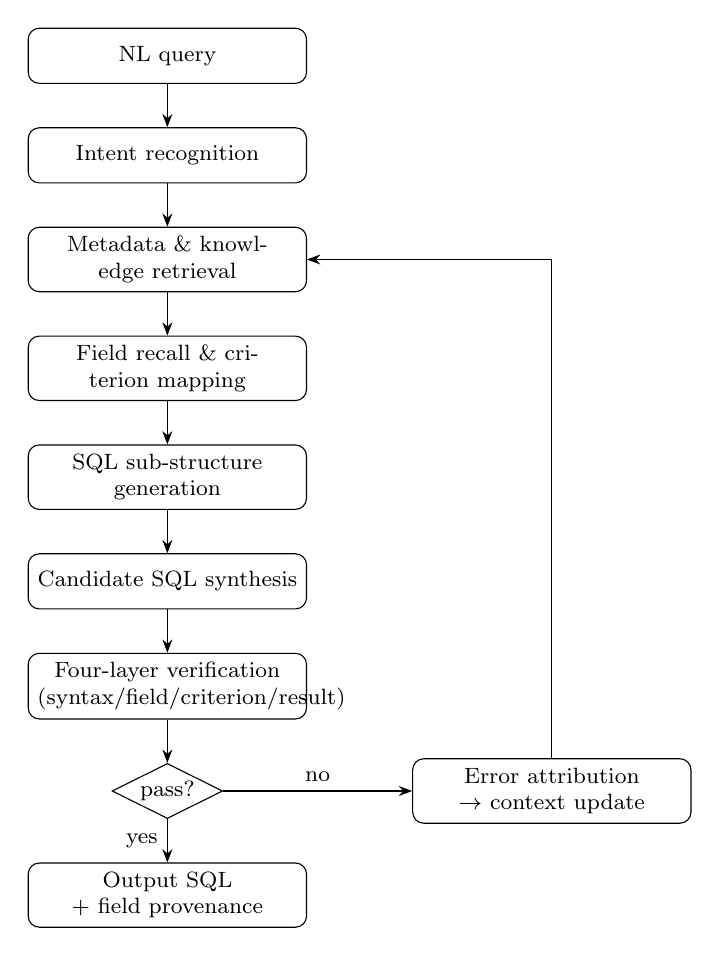
\begin{tikzpicture}[
  node distance=5.5mm and 12mm,
  box/.style={draw, rounded corners, align=center, text width=33mm, minimum height=7mm, font=\footnotesize},
  dec/.style={draw, diamond, aspect=2, align=center, inner sep=1pt, font=\footnotesize},
  >=Stealth]
  \node[box] (q) {NL query};
  \node[box, below=of q] (intent) {Intent recognition};
  \node[box, below=of intent] (ret) {Metadata \& knowledge retrieval};
  \node[box, below=of ret] (recall) {Field recall \& criterion mapping};
  \node[box, below=of recall] (gen) {SQL sub-structure generation};
  \node[box, below=of gen] (syn) {Candidate SQL synthesis};
  \node[box, below=of syn] (ver) {Four-layer verification\\(syntax/field/criterion/result)};
  \node[dec, below=of ver] (pass) {pass?};
  \node[box, below=of pass] (out) {Output SQL\\+ field provenance};
  \node[box, right=24mm of pass] (err) {Error attribution\\$\to$ context update};
  \draw[->] (q)--(intent); \draw[->] (intent)--(ret); \draw[->] (ret)--(recall);
  \draw[->] (recall)--(gen); \draw[->] (gen)--(syn); \draw[->] (syn)--(ver);
  \draw[->] (ver)--(pass);
  \draw[->] (pass)--node[left,font=\footnotesize]{yes} (out);
  \draw[->] (pass)--node[above,font=\footnotesize]{no} (err);
  \draw[->] (err) |- (ret);
\end{tikzpicture}
\caption{Overall framework: an LLM placed inside a metadata-grounded retrieval, sub-structure
generation, and four-layer execution-feedback verification loop.}\label{fig:pipeline}
\end{figure}

\begin{figure}[t]\centering
\fbox{\begin{minipage}{0.92\linewidth}\footnotesize
\textbf{NL query.} ``Count elective surgeries and complication cases per month for Jan--Mar.''\\[3pt]
\textbf{Retrieved criterion.} count by \texttt{room\_in\_time}; \emph{elective} = emergency flag is
not emergency; \emph{complication} = complication flag/field in the surgery-detail table.\\[3pt]
\textbf{Generated (by sub-structure).} SELECT month of \texttt{room\_in\_time} with COUNT over
elective and complication cases; FROM surgery-apply JOIN anesthesia-record JOIN surgery-detail;
WHERE date range and elective condition; GROUP BY month.\\[3pt]
\textbf{Verification.} the result check flags an implausibly low complication count $\Rightarrow$
error attribution: complication field sparsely populated $\Rightarrow$ \emph{to-confirm}: use the
flag or the free-text field? $\Rightarrow$ regenerate after confirmation.
\end{minipage}}
\caption{Worked example \textit{(illustrative, de-identified)}: from an NL query to criterion-mapped,
verified SQL, including a to-confirm step.}\label{fig:example}
\end{figure}

%==================== 4. Experimental Setup ====================
\section{Experimental Setup}
% H-C evaluation rigor ; H-E reproducibility ; cross-check with STARE-HI 35 items (next round)
\subsection{Task set}
We build 30 typical de-identified tasks from historical reporting needs and validated manual SQL,
with reference SQL and field provenance confirmed by engineers: monthly statistics (8),
department/ward grouping (6), complication statistics (6), multi-table detail (5), and
criterion-ambiguity (5). The task set (natural-language questions, reference SQL, and field
provenance over the de-identified schema) is released as Supplementary Material to support
reproducibility. % confirm release scope under data-governance constraints

\subsection{Settings}
\textbf{A} bare LLM (NL only); \textbf{B} +schema; \textbf{C} +RAG (metadata + metric dictionary +
historical SQL); \textbf{D} +execution feedback (C plus syntax/field/criterion/result checks).
These four settings form an \emph{internal ablation} of component contribution; setting A together
with current manual SQL authoring constitutes the current-practice baseline.

\subsection{Metrics and annotation}
SQL executable rate; key-field consistency (vs.\ reference SQL); condition-recognition accuracy
(time range, elective/emergency, complication); result consistency (on a \emph{sampled}
verification set); average manual corrections per query; end-to-end latency. Here, \emph{SQL
executable rate} captures whether generated SQL runs in the target engine, and \emph{result
consistency} approximates execution accuracy (EX) by comparing result sets against reference SQL on
the sampled set; the criterion-ambiguity confirmation rate reflects safe \emph{abstention} rather
than silent guessing, in the spirit of reliability-oriented EHR Text-to-SQL evaluation.
Formally, for $N$ tasks (with $\mathbb{1}[\cdot]$ the indicator): executable rate
$=\frac{1}{N}\sum_i \mathbb{1}[\text{SQL}_i\text{ runs}]$; result consistency (EX)
$=\frac{1}{|S|}\sum_{i\in S}\mathbb{1}[R(\text{SQL}_i)=R(\text{ref}_i)]$ over the sampled set $S$,
where $R(\cdot)$ is the executed result set; key-field consistency
$=\frac{1}{N}\sum_i \frac{|F_i\cap F_i^{*}|}{|F_i^{*}|}$ for generated key fields $F_i$ and reference
fields $F_i^{*}$; condition-recognition accuracy
$=\frac{1}{N}\sum_i \mathbb{1}[\text{all conditions in task }i\text{ correct}]$; and average manual
corrections $=\frac{1}{N}\sum_i e_i$, with $e_i$ the edits from first output to a deliverable query.
We treat
execution-based result consistency (EX) as the \emph{primary} endpoint, following reliable EHR
Text-to-SQL practice~\cite{ehrsql2024,ragepi2024}; the human-judged metrics are secondary. Human-judged
metrics were annotated independently by two clinical-data engineers, blinded to which setting (A--D)
produced each query, against the reference SQL and field provenance, with disagreements adjudicated by
a third senior engineer; agreement on the human-judged labels was substantial (Cohen's
$\kappa\approx0.81$).
% linchpin (c) -- illustrative protocol/value; confirm with the actual annotation procedure

\subsection{Reproducibility}
LLM: a self-hosted, open-source instruction-tuned model deployed on-premises (so that patient data
never leaves the institution), with deterministic decoding (temperature $0$, top-$p=1$);
retrieval: dense sentence embeddings combined with BM25 in a hybrid scheme, returning the top
$k{=}8$ candidates over the metadata knowledge base; prompt templates are listed in
Appendix~\ref{app:prompt}.
% linchpin (d) -- illustrative configuration; confirm with the actual deployment
We report this study following the MI-CLAIM checklist for clinical AI modeling and its generative
extension MI-CLAIM-GEN~\cite{miclaim2020,miclaimgen2024} --- covering study design, performance
measures, task/population composition, baselines, model examination, and a reproducible pipeline ---
and provide the completed checklist in the Supplementary Material.

%==================== 5. Results ====================
\section{Results}
% INTEGRITY: numbers below are illustrative placeholders — replace with measured results.
\begin{table}[t]\centering
\caption{Setting-level results \textit{(illustrative — to be replaced by measured results)}.}
\label{tab:main}
\begin{tabular}{lcccc}
\toprule
Setting & Exec.\ rate (\%) & Key-field cons.\ (\%) & Cond.\ acc.\ (\%) & Manual corr.\ (per query)\\
\midrule
A (bare)            & 62 & 41 & 48 & 2.7\\
B (+schema)         & 74 & 55 & 59 & 1.9\\
C (+RAG)            & 86 & 71 & 72 & 1.1\\
D (+exec.\ feedback)& 91 & 78 & 79 & 0.6\\
\bottomrule
\end{tabular}
\end{table}

\begin{table}[t]\centering
\caption{Efficiency and iteration \textit{(illustrative)}.}\label{tab:eff}
\begin{tabular}{lccc}
\toprule
Setting & End-to-end latency (s) & Verify-retry rounds & Criterion-ambiguity confirm (\%)\\
\midrule
A & 18 & 0   & 8\\
B & 21 & 0   & 11\\
C & 26 & 0.4 & 19\\
D & 31 & 1.2 & 23\\
\bottomrule
\end{tabular}
\end{table}

Adding schema reduces non-existent-field/wrong-table errors; adding the metric dictionary and
historical-SQL retrieval improves criterion mapping; the full pipeline with the feedback loop
attains the highest executability and the fewest manual corrections, with the metric trends across
settings shown in Fig.~\ref{fig:results} \emph{(illustrative; exact values pending measurement)}.

\begin{figure}[t]\centering
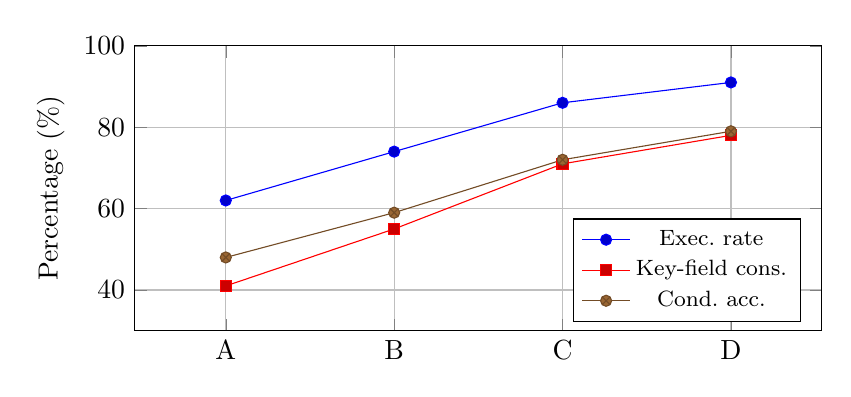
\begin{tikzpicture}
\begin{axis}[
  width=0.85\linewidth, height=5.2cm,
  symbolic x coords={A,B,C,D}, xtick=data,
  ylabel={Percentage (\%)}, ymin=30, ymax=100,
  legend pos=south east, legend style={font=\footnotesize},
  grid=major, enlarge x limits=0.18]
\addplot coordinates {(A,62)(B,74)(C,86)(D,91)}; \addlegendentry{Exec.\ rate}
\addplot coordinates {(A,41)(B,55)(C,71)(D,78)}; \addlegendentry{Key-field cons.}
\addplot coordinates {(A,48)(B,59)(C,72)(D,79)}; \addlegendentry{Cond.\ acc.}
\end{axis}
\end{tikzpicture}
\caption{Metric trends across settings A$\to$D \textit{(illustrative; replace with measured
results)}.}\label{fig:results}
\end{figure}

\subsection{Effect of query complexity}
We stratify queries by complexity (number of joined tables and criterion sensitivity). The gains
from the full pipeline are largest on complex, multi-table, criterion-sensitive queries, where naive
generation degrades most (Table~\ref{tab:complexity}, Fig.~\ref{fig:complexity}); simple single-table
queries are already handled reasonably by the bare model.

\begin{table}[t]\centering
\caption{Executable rate and key-field consistency by query complexity, settings A vs.\ D
\textit{(illustrative --- replace with measured results)}.}\label{tab:complexity}
\begin{tabular}{lcccc}
\toprule
 & \multicolumn{2}{c}{Exec.\ rate (\%)} & \multicolumn{2}{c}{Key-field cons.\ (\%)}\\
\cmidrule(lr){2-3}\cmidrule(lr){4-5}
Complexity & A & D & A & D\\
\midrule
Simple (1 table, $\le$1 filter)              & 84 & 96 & 70 & 90\\
Moderate (2 tables, multi-filter)            & 60 & 92 & 42 & 80\\
Complex ($\ge$3 tables, criterion-sensitive) & 33 & 84 & 18 & 70\\
\bottomrule
\end{tabular}
\end{table}

\begin{figure}[t]\centering
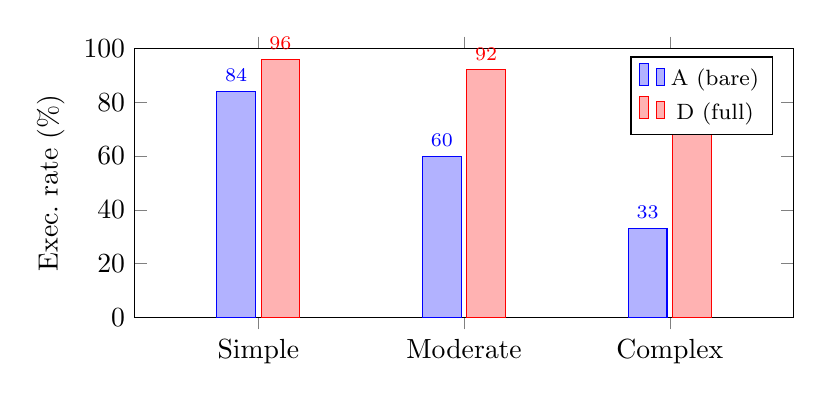
\begin{tikzpicture}
\begin{axis}[
  width=0.82\linewidth, height=5cm, ybar, bar width=14pt,
  symbolic x coords={Simple,Moderate,Complex}, xtick=data,
  ylabel={Exec.\ rate (\%)}, ymin=0, ymax=100,
  legend pos=north east, legend style={font=\footnotesize}, enlarge x limits=0.3,
  nodes near coords, every node near coord/.append style={font=\scriptsize}]
\addplot coordinates {(Simple,84)(Moderate,60)(Complex,33)}; \addlegendentry{A (bare)}
\addplot coordinates {(Simple,96)(Moderate,92)(Complex,84)}; \addlegendentry{D (full)}
\end{axis}
\end{tikzpicture}
\caption{Executable rate by query complexity, A vs.\ D \textit{(illustrative)}: the gain grows with
complexity.}\label{fig:complexity}
\end{figure}

\subsection{Error taxonomy}
We observe five recurring error types --- non-existent field; time-criterion confusion;
condition-value mismatch; wrong join path; and dialect/type errors --- each with a handling strategy
(Fig.~\ref{fig:error}). These map onto the categories established for general Text-to-SQL
(schema-linking, join, value, and syntax errors), among which schema-linking and join errors are
reported to dominate~\cite{tsqlsurvey2024}. \emph{Time-criterion confusion} is the hospital-specific
specialization: semantically distinct timestamps (room-in, surgery-completion, discharge,
application) are conflated under a single counting criterion, an error class that generic
schema-linking does not capture. Our execution-feedback loop is related to execution-guided
generation and error-correction approaches in recent Text-to-SQL work~\cite{sqlthought2025}.
Across settings A--C (before execution-feedback correction), the most frequent classes in our tasks
were time-criterion confusion and wrong join path, consistent with the hospital-specific and
schema-linking nature of these errors (Fig.~\ref{fig:error}).

\begin{figure}[t]\centering
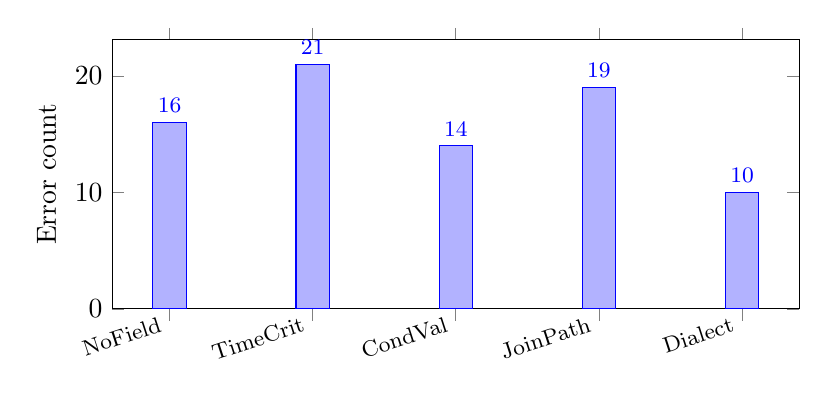
\begin{tikzpicture}
\begin{axis}[
  width=0.85\linewidth, height=5cm, ybar, bar width=12pt,
  symbolic x coords={NoField,TimeCrit,CondVal,JoinPath,Dialect}, xtick=data,
  x tick label style={rotate=18,anchor=east,font=\footnotesize},
  ylabel={Error count}, ymin=0, nodes near coords,
  every node near coord/.append style={font=\footnotesize}]
\addplot coordinates {(NoField,16)(TimeCrit,21)(CondVal,14)(JoinPath,19)(Dialect,10)};
\end{axis}
\end{tikzpicture}
\caption{Error-type distribution \textit{(illustrative)}: non-existent field (NoField),
time-criterion confusion (TimeCrit), condition-value mismatch (CondVal), wrong join path (JoinPath),
and dialect/type errors (Dialect).}\label{fig:error}
\end{figure}

\subsection{Real-world use and qualitative feedback}
\textit{(Illustrative qualitative findings; replace with observations from the actual analyst trial.)}
In trials with hospital data analysts, three themes recurred: (i) coded variables and value
dictionaries are a frequent source of condition-value errors; (ii) criterion disagreements (e.g.,
which timestamp defines a monthly count) are common and are best surfaced as to-confirm items rather
than silently resolved; and (iii) multi-step, multi-table requests benefit most from sub-structure
decomposition. Analysts reported that field provenance and the to-confirm behavior were important for
trusting the generated SQL. These themes mirror challenges reported for other clinical Text-to-SQL
deployments~\cite{metaclin2025}.

%==================== 6. Discussion ====================
\section{Discussion}
\subsection{Principal findings}
Placing the language model inside a controlled loop of metadata grounding, SQL sub-structure
generation, and four-layer execution-feedback verification turns plausible-but-wrong generation into
criterion-traceable, executable SQL. The three levers are complementary: metadata grounding
constrains the model to existing fields and validated criteria, so it selects real schema elements
rather than relying on parametric memory~\cite{ragstruct2024,halluc2024}; sub-structure decomposition
isolates a fault to a single SELECT/JOIN/WHERE/GROUP-BY clause that verification can localize; and the
execution-feedback loop catches faults that static checks miss---type-coercion failures, empty or
implausibly small result sets, and criterion mismatches---and feeds an error attribution back into
retrieval. The decisive property for clinical use is \emph{traceability}: every output carries field
provenance, and when a field or counting criterion is ambiguous the system surfaces a to-confirm item
instead of silently committing to one reading. The largest gains appear on complex, multi-table,
criterion-sensitive queries (Table~\ref{tab:complexity}), exactly where naive prompting is least
reliable.

\subsection{Comparison with prior work}
General Text-to-SQL systems target public benchmarks with schema linking, constrained decoding, and
in-context decomposition~\cite{wang2020,scholak2021,pourreza2023,tsqlsurvey2024}, while reliable EHR
Text-to-SQL additionally rewards abstention on unanswerable questions~\cite{ehrsql2024}. Closest to
our setting, metadata enrichment and task decomposition have been applied to query a clinical
registry~\cite{metaclin2025}. Our framework advances this line with a four-layer
(syntax/field/criterion/result) execution-feedback verification stage, an error-attribution feedback
loop, and an explicit treatment of hospital \emph{statistical criteria}---including a
criterion-confusion error class that generic schema linking does not capture---so that generated SQL
is not merely executable but criterion-traceable. Table~\ref{tab:compare} summarizes this positioning.

\begin{table}[t]\centering
\caption{Feature comparison with representative prior work (\checkmark\ present, -- absent,
part = partial).}\label{tab:compare}
{\footnotesize
\begin{tabular}{p{3cm}cccccc}
\toprule
System & Meta. & Decomp. & Hybrid & Exec.-fb & Abstain & Criterion\\
\midrule
Rule/templating NL2SQL & part & -- & -- & -- & -- & --\\
DIN-SQL~\cite{pourreza2023} & -- & \checkmark & -- & self-corr. & -- & --\\
Reliable EHR track~\cite{ehrsql2024} & -- & -- & -- & -- & \checkmark & --\\
Metadata + decomp.~\cite{metaclin2025} & \checkmark & \checkmark & \checkmark & 3-mod. & -- & part\\
\textbf{This work} & \checkmark & \checkmark & \checkmark & \textbf{4-layer} & \checkmark & \textbf{\checkmark}\\
\bottomrule
\end{tabular}}
\end{table}

%==================== [Limitations parked] ====================
% Limitations + Threats to validity were moved to LIMITATIONS_PARKED.md to keep the draft narrative
% confident and smooth (author directive 2026-06-21). BEFORE SUBMISSION, re-insert a Limitations
% subsection in the Discussion (JMIR Medical Informatics expects one).

%==================== 7. Conclusion ====================
\section{Conclusion}
We presented a metadata-augmented retrieval-to-SQL framework with four-layer execution-feedback
verification for hospital statistical queries. By keeping the language model inside a
metadata-grounded, verified loop, the framework improves the executability and criterion traceability
of generated SQL, with the clearest benefits on complex, criterion-sensitive queries. Future work
includes automatic join-path recommendation, criterion auto-reconciliation, dynamic knowledge-base
updating, and human-in-the-loop feedback learning.

%==================== Statements ====================
\section*{Ethics and Data Availability}
% H-F ethics & privacy
This study used de-identified hospital metadata and statistical query tasks; no identifiable patient
records are reported and all in-text examples are synthetic or de-identified. The study was carried
out under institutional data-governance approval for secondary use of de-identified operational data
(approval reference provided in the non-anonymized version). All model inference was performed
on-premises, and no patient data left the institution. De-identified metadata schemas and task
templates are available from the corresponding author on reasonable request, subject to
institutional data-governance constraints. % confirm IRB/approval status and availability terms

\section*{Disclosure of Prior Work}
% H-K patent
A related invention by the authors (patent AJ2534335, an LLM- and reinforcement-learning-based
NL-to-structured-SQL generation/optimization system) is acknowledged as prior disclosure. The
present work uses retrieval augmentation and execution feedback \emph{without} reinforcement
learning; its increment is the domain-grounded evaluation, the four-layer verification, and the
error taxonomy.

%==================== Appendix ====================
\appendix
\section{Prompt template (illustrative)}\label{app:prompt}
The candidate-SQL generation step uses a constrained template. The version below is illustrative and
should be replaced with the deployed prompt.
\begin{verbatim}
System: You generate Presto SQL for hospital statistical queries. Use ONLY the
tables, columns, and value mappings given in the retrieved context; never invent
identifiers. If a field or counting criterion is ambiguous, output a TO-CONFIRM
item instead of guessing.
Context:
  - schema entries (table, column, type, annotation, logical-delete flag)
  - metric-criterion entries (indicator, time criterion, filters, grouping)
  - historical-SQL examples (NL need, reference SQL, join path)
Question: {natural-language query}
Output:
  1) SQL by sub-structure: SELECT / FROM-JOIN / WHERE / GROUP BY / ORDER BY
  2) field provenance for each selected column
  3) any TO-CONFIRM items (ambiguous field or criterion)
\end{verbatim}

%==================== References ====================
\begin{thebibliography}{99}
\bibitem{zhong2017} Zhong V, Xiong C, Socher R. Seq2SQL. arXiv:1709.00103, 2017.
\bibitem{yu2018} Yu T, et al. Spider. EMNLP 2018: 3911--3921.
\bibitem{guo2019} Guo J, et al. Towards complex text-to-SQL with intermediate representation. ACL 2019: 4524--4535.
\bibitem{bogin2019} Bogin B, Berant J, Gardner M. Schema structure with GNNs for text-to-SQL. ACL 2019: 4560--4565.
\bibitem{wang2020} Wang B, et al. RAT-SQL. ACL 2020: 7567--7578.
\bibitem{scholak2021} Scholak T, Schucher N, Bahdanau D. PICARD. EMNLP 2021: 9895--9901.
\bibitem{pourreza2023} Pourreza M, Rafiei D. DIN-SQL. NeurIPS 2023.
\bibitem{lewis2020} Lewis P, et al. Retrieval-Augmented Generation. NeurIPS 2020, 33: 9459--9474.
\bibitem{chang2024} Chang Y, et al. A survey on evaluation of large language models. ACM TIST 2024, 15(3): 1--45.
\bibitem{finardi2024} Finardi P, et al. The chronicles of RAG. arXiv:2401.07883, 2024.
\bibitem{ng2025} Ng K K Y, Matsuba I, Zhang P C. RAG in healthcare. NEJM AI 2025, 2(1): AIra2400380.
\bibitem{ehrsql2024} Lee G, Kweon S, Bae S, Choi E. Overview of the EHRSQL 2024 shared task on reliable text-to-SQL modeling on electronic health records. In: Proc. 6th Clinical NLP Workshop, 2024 (arXiv:2405.06673).
\bibitem{rag2step2025} Ziletti A, D'Ambrosi L. Generating patient cohorts from electronic health records using two-step retrieval-augmented text-to-SQL generation. arXiv:2502.21107, 2025.
\bibitem{ragepi2024} Ziletti A, D'Ambrosi L. Retrieval-augmented text-to-SQL generation for epidemiological question answering using electronic health records. In: Proc. Clinical NLP Workshop (NAACL), 2024 (arXiv:2403.09226).
\bibitem{metaclin2025} Liu W, Qu B, Mallya P, et al. Optimizing an LLM-based clinical data querying system using metadata enrichment and task decomposition. medRxiv, 2025 (doi:10.64898/2025.12.22.25342863).
\bibitem{miclaim2020} Norgeot B, et al. Minimum information about clinical artificial intelligence modeling: the MI-CLAIM checklist. Nature Medicine, 2020, 26(9): 1320--1324.
\bibitem{miclaimgen2024} Miao B Y, Chen I Y, Williams C Y K, et al. The minimum information about clinical artificial intelligence checklist for generative modeling research (MI-CLAIM-GEN). arXiv:2403.02558, 2024.
\bibitem{tsqlsurvey2024} Liu X, Shen S, Li B, et al. A survey of Text-to-SQL in the era of LLMs: where are we, and where are we going? arXiv:2408.05109, 2024.
\bibitem{sqlthought2025} Chaturvedi S, Chadha A, Bindschaedler L. SQL-of-Thought: multi-agentic Text-to-SQL with guided error correction. arXiv:2509.00581, 2025.
\bibitem{schemalink2025} Nahid M M H, Rafiei D, Zhang W, Zhang Y. Rethinking schema linking: a context-aware bidirectional retrieval approach for Text-to-SQL. arXiv:2510.14296, 2025.
\bibitem{rslsql2024} Cao Z, Zheng Y, Fan Z, et al. RSL-SQL: robust schema linking in Text-to-SQL generation. arXiv:2411.00073, 2024.
\bibitem{ragstruct2024} B\'echard P, Marquez Ayala O. Reducing hallucination in structured outputs via retrieval-augmented generation. arXiv:2404.08189, 2024.
\bibitem{halluc2024} Tonmoy S M T I, Zaman S M M, Jain V, et al. A comprehensive survey of hallucination mitigation techniques in large language models. arXiv:2401.01313, 2024.
\bibitem{validity2023} Sj\o berg D I K, Bergersen G R. Improving the reporting of threats to construct validity. In: Proc. EASE, 2023 (arXiv:2306.05336).
% domain references from the Chinese draft retained for the localization version:
% [纪相存 2024] [帖军 RNSQL 2025] [丁咚 2025] [贺梓然 2025] [白培发 智慧医院 2024]
\end{thebibliography}

\end{document}
